\chapter{Hardware}

\section{El circuito del TransistorTester}
\label{sec:hardware}

El circuito del  TransistorTester que aparece en  la figura \ref{fig:ttester} se basa  en el circuito de  Markus F. que.
\cite{Frejek} ha publicado en la fig.~1 de su informe AVR-Transistortester Los componentes o partes movidos o cambiados.
están marcados con el color verde, las partes opcionales están marcadas con el color rojo                            .

Algunos  cambios se  han llevado  a cabo  porque el  interruptor electrónico  de corriente  causa problemas  en algunas
implementaciones. Por  tanto la resistencia  R7 se ha  reducido a un  valor de \(3,3k\Omega\).  El condensador C2  se ha
reducido a 10nF y R8 se  ha movido, de manera que la salida PD6 no intente  descargar el condensador C2 directamente. Se
han añadido  condensadores de  desacoplado y deben  colocarse cerca  de la fuente  de energía del  ATmega y  cerca del
regulador de voltaje.

Debido a que los únicos pines que necesitan resistencias  con PD7 y PC6 (RESET), una resistencia extra \(27k\Omega\) se
añade  a la  entrada PD7  (pin~13). Con  esta modificación,  el software  puede desactivar  todas las  resistencias de
polarización (pull-up) del ATmega.

Opcionalmente, se puede añadir un cristal de cuarzo con sus  condensadores de 22pF La precisión de un cristal trae el.
beneficio de una medida de tiempo más estable para obtener los valores de los condensadores                           .

La nueva  versión del  software puede usar  el interruptor  de escalado de  voltaje de la  fuente de  alimentación. La
velocidad de  conmutación se  reduce gracias al  condensador externo  C1 que está  conectado al pin  de AREF  (21) del
ATmega. Para prevenir  una medición más lenta de la  necesaria, el valor de este condensador  debería reducirse hasta
1nF. También  es posible  quitar el condensador  C1. Para  adaptar el software  al circuito actual  habrá que  echa un
vistazo a las opciones del fichero Makefile en el capítulo sobre la configuración \ref{sec:config}.

Por Internet circulan algunas versiones distintas de combinaciones de resistencias R11 / R12. He adaptado mi software al
original de Markus F. \cite{Frejek} con resistencias de \(10k\Omega\) y \(3,3k\Omega\).

La referencia  de tensión de  precisión adicional  de 2.5V en  el pin PC4  (ADC4) se  puede utilizar para  comprobar y
calibrar la tensión VCC, aunque no es obligatoria.  También se puede utilizar un LM4040AIZ2.5 (0.1\%), un LT1004CZ-2.5
(0.8\%) o un LM336-Z2.5 (0.8\%) como referencia de tensión. Si  no se instala la referencia de tensión de precisión y
no  se quiere  añadir una  extensión de relé,  se debería  instalar una  resistenca
\texttt{pull up}  R16 a PC4  con una resistencia  de gran valor  (\(47k\Omega\)). Esto ayuda  al software a  detectar la
referencia de tensión que falta. Se ha añadido un conector opcional ISP para facilitar la carga de nuevas versiones de
software al tester.

\begin{figure}[H]
\centering

\includegraphics[width=18cm]{../FIG/ttester.eps}
\caption{El nuevo circuito del TransistorTester}
\label{fig:ttester}
\end{figure}

El software puede seguir a otra asignación de pines del puerto  D para una conexión más simple de la pantalla LCD. La
siguiente tabla \ref{tab:grid-change} muestra las modificaciones de  las asignaciones para disposición de la rejilla de
líneas y la conexión  de una pantalla gráfica para microcontroladores ATmega8/168/328. También  se muestra el uso de
entradas de puertos para funciones adicionales. Con las conexiones para la pantalla gráfica con opción de disposición
de rejilla de  líneas (STRIP\_GRID\_BOARD) no se puede usar  la función del contador de frecuencias,  porque el puerto
PD4 (T0) está en uso. Pero esta conexión sí se usa en una versión china con pantalla gráfica.


\begin{table}[H]
  \begin{center}
    \begin{tabular}{| c || c | c | c | c | c |}
    \hline
           & carácter LCD & carácter LCD    & ST7565 LCD & ST7565 LCD       & función adicional \\
      Puerto &               & placa de rejilla de líneas &            & placa de rejilla de líneas &  \\
    \hline
    \hline
    PD0    &  LCD-D4       &  pulsador      &  LCD-REST    &                  &  \\
    \hline
    PD1    &  LCD-D5       &  LCD-D7        &  LCD-RS      & LCD-SI           & codificador rotatorio 2  \\
    \hline
    PD2    &  LCD-D6       &  LCD-D6        &  LCD-SCLK    & LCD-SCLK         &  \\
    \hline
    PD3    &  LCD-D7       &  LCD-D5        &  LCD-SI      & LCD-A0 (RS)      & codificador rotatorio 1 \\
    \hline
    PD4    &  LCD-RS       &  LCD-D4        &              & LCD-REST         & contador de frecuencias \\
    \hline
    PD5    &  LCD-E        &  LCD-E         &              &                  &  \\
    \hline
    PD7    &  pulsador     &  LCD-RS        &              &                  &  \\
    \hline
    \end{tabular}
  \end{center}
  \caption{Different variations of the display port assignments}
  \label{tab:grid-change}
\end{table}


\subsection{Protección de las entradas del ATmega}

Para mejorar la protección de las entradas del ATmega, uno de los circuitos adicionales~ \ref{fig:relay_addon} se puede
integrar. Los contactos sin carga del relé protege el ATmega sin corriente. Los contactos se abrirán mediante software
únicamente  para medición.  También con  protección  adicional de  un diodo  la  posibilidad de  proteger el  ATmega
mejorará frente a la conexión de un condensador con  tensión residual muy alta. Pero no será posible una protección
completa. Además, los condensadores deben descargarse antes de proceder a la medición.

\begin{figure}[H]
  \begin{subfigure}[b]{9cm}
    \centering
    
\includegraphics[width=7cm]{../FIG/relay_addon.eps}
    \caption{con relé}
  \end{subfigure}
  ~
  \begin{subfigure}[b]{9cm}
    \centering
    
\includegraphics[width=7cm]{../FIG/diode_addon.eps}
    \caption{con diodos}
  \end{subfigure}
  \caption{Protección adicional de las entradas del ATmega}
  \label{fig:relay_addon}
\end{figure}

\subsection{Medición de tensión de un diodo zener por encima de 4 Volt}

Si no se requiere la salida  serie de texto, el pin PC3 del ATmega se puede usar  como entrada analógica para medir una
tensión externa. La tensión puede  llegar hasta 50V con un divisor de resistencias 10:1 opcional  y se puede usar para
medir la caída de tensión de un diodo zener. Una fuente de alimentación limitada actualmente a 50V puede conmutarse a
una señal baja en el pin PD7 del ATmega para suministrar corriente con el fin de comprobar la tensión de ruptura de un
diodo zener. La Figura~\ref{fig:zener} muestra una sugerencia para  esta expansión. El tester marca la tensión externa
durante todo el tiempo que se mantenga presionado el botón. Alrededor de 40mA más de corriente de batería se usa para
esta expansión durante el tiempo en que se presiona el botón.

\begin{figure}[H]
\centering

\includegraphics[width=12cm]{../FIG/zener_exp.eps}
\caption{Expansion for measuring of break down voltage of Zener diodes}
\label{fig:zener}
\end{figure}

El divisor de tensión se puede usar con la parte opcional de diálogo para el ATmega328 sin el conversor DC-DC activado
para medir  el diodo zener.  Si la tecla no  está presionada el  conversor de tensión  no está encendido. Por  eso la
tensión externa  (por ejemplo, la tensión  de una batería) pueda  ser medida en el  puerto del diodo zener.  Sólo se
pueden medir corrientes continuas positivas de gasta 50V. No se debe olvidar que hay que tener en cuenta la polaridad.

\subsection{Generador de frecuencias}

Con la  parte de diálogo  del ATmega328 podemos  seleccionar un generador de  frecuencias, que soporta  actualmente una
selección de frecuencias desde  \(1 Hz\) hasta \(2 MHz\). La salida  de la señal de 5V se hace  con una resistencia de
\(680\Omega\) conectada al puerto  de test TP2. Podemos usar la  señal de tierra desde el cátodo  (pin negativo) de la
extensión del diodo zener o el puerto de test de TP1. El  puerto de test TP3 se conecta a tierra con una resistencia de
\(680\Omega\).

\subsection{Medición de frecuencias}

Igualmente para usarlo con el diálogo seleccionable la  medición de frecuencias es una pequeña extensión de hardware
necesaria. El ind de  entrada PD4 /T0/PCINT20) del ATmega se  usa para la medición de frecuencias. El  mismo pin se usa
también para conectarlo a  la pantalla LCD. Con una disposición  normal, el PD4 se conecta a la  señal LCD-RS, con el
diseño de la disposición de  rejilla de líneas. Para ambas señales el pin PD4 puede  conmutarse a la entrada todo el
tiempo que  no se  requiera una salida  a la  LCD. La pantalla  LCD sólo  es interesante respecto  al valor  de entrada
únicamente, si  la señal  LCD-E está conectada  a tierra.  Para controlar el  pin de entrada  desde un  reloj externo
deberá usarsa  el menos una  resistencia en serie  de \(270\Omega\).  Es más recomendable  utilizar el circuito  de la
figura~\ref{fig:FreqMes}. La  tensión del  pin PD4  (LCD-RS or  LCD-D4) se debería  ajustar a  \(2.4V\) sin  el ATmega
ensamblado o  durante la medicion  de la frecuencia  del ATmega, para  obtener la mejor  sensibilidad para la  señal de
frecuencia de entrada. La pantalla LCD siempre debería estar instalado para ajustarlo, porque la resistencia pull up de
la LCD cambia la tensión.

\begin{figure}[H]
\centering

\includegraphics[width=7cm]{../FIG/Frequency_addon.eps}
\caption{Extensión para la medición de la frecuencia}
\label{fig:FreqMes}
\end{figure}

\subsection{Utilización de un codificador de pulsos rotatorio}

Para  controlar mas  fácilmente la  función del  menú  para el  ATmega328 podemos  expandir el  circuito mediante  un
codificador de pulsos  rotatorio con un botón  pulsador. El circuito~\ref{fig:RotExt} muestra  una expansión estándar
para una pantalla  de caracteres normal LCD.  Todas las señales para  laa conexión de codificador  de pulsos rotatorio
están disponibles en el conector  de la LCD. Por esta razón la expansión se  puede actualizar fácilmente para muchos
testers existentes. En muchos casos la LCD gráfica se ensambla sobre un adaptador con algunas conexiones de la pantalla
LCD de caracteres. También en estos casos la actualización con un codificador rotatorio no presenta dificultad.

\begin{figure}[H]
\centering

\includegraphics[width=6cm]{../FIG/rotary_extension.eps}
\caption{Expansión con un codificador de pulsos rotatorio}
\label{fig:RotExt}
\end{figure}

La figura~\ref{fig:RotEnc} muestra las características de dos  codificadores de pulsos rotatorios distintos. La primera
versión tiene  el doble  de veces  de cantidad de  posiciones indexadas  (\textit{\color{red}{detents}}) por  turno que
pulsos por turno. La segunda  versión tiene el mismo número de posiciones indexadas que  pulsos por turno. El descenso
de una  de las dos señales  que conmutan está a  veces exactamente en la  misma posición indexada del  codificador de
pulsos rotatorio.

\begin{figure}[H]
\centering

\includegraphics[width=14cm]{../FIG/rotary_encoder.eps}
\caption{Características de dos  codificadores de pulsos rotatorios distintos}
\label{fig:RotEnc}
\end{figure}

La figura~\ref{fig:RotBounce}  muesta un codificador de  pulsos rotatorio, que  no sólo tiene contactos  rígidos, pero
también tiene un  estado inestable de uno de los  interruptores en la posición indexada. Cada  cambiodel estado de los
interruptores lo detecta el programa  guardado en un \textit{buffer} cíclico. Por eso los  tres últimos estados de los
interruptores se pueden comprobar después de cada cambio de estado.

Para cada  ciclo de  estados conmutados  se pueden  definir un total  de cuatro  secuencias para  cada dirección  de la
rotación. Si sólo hay una posición indexada para cada ciclo de estados conmutados, sólo uno del par de secuencias de
estados  debe  ser vigilado  (\texttt{WITH\_ROTARY\_SWITCH=2}  ó  \texttt{3}) para  una  cuenta  correcta. Si  hay  dos
posiciones indexadas para cada  ciclo de estados conmutados, como se muestra en  la figura~\ref{fig:RotBounce}, se deben
vigilar  los pares  de secuencias  de estados  conmutados (\texttt{WITH\_ROTARY\_SWITCH=1}).  Se puede  elegir cualquier
resolución para  (\texttt{WITH\_ROTARY\_SWITCH} para un  codificador de pulsos  rotatorio sin posiciones  indexadas. Un
valor de 2 ó 3 selecciona la resolución más baja, un valor de 1 selecciona una resolución media y de 5 selecciona la
resolución más alta. Una oscilación de la selección (Una subida o bajada del contador) se puede prevenir con el tipo
de selección de monitorización, pero a veces se puede perder  una cuenta debido a una mala colocación de la posición
indexada.

\begin{figure}[H]
\centering

\includegraphics[width=14cm]{../FIG/rotary_bouncing.eps}
\caption{Codificador de pulsos rotatorios con conmutadores rígidos}
\label{fig:RotBounce}
\end{figure}

En lugar de  los dos conmutadores de un codificador  de pulsos rotatorios también podemos instalar  dos teclas para los
mover hacia arriba y hacia abajo, si no hay un codificador presente. En ese caso la opción WITH\_ROTARY\_SWITCH deberá
valer 4 para una manejo correcto del programa.

\subsection{Conexión de una pantalla gráfica}

Quiero agradecer a Wolfgang Sch. por su trabajo en el soporte de una versión china con el controlador ST7565. Por ahora
se puede conectar  una pantalla gráfica LCD  de 128x64 píxeles con un  controlador ST7565. Ya que  este controlador se
conecta a un interfaz  serie, sólo son necesarias cuatro líneas  para la señal. En otro caso se  pueden dos pines del
puerto D del ATmega. El procesador del ATmega debería  tener al menos 32K de memoria \textit{flash} para poder soportar
una pantalla  gráfica. El controlador ST7565  funciona con una  tensión operativa de  3,3V. Por tanto, se  requiere un
regulador de tensión  de 3,3V. La hoja de especificaciones  del controlador ST7565 no permite la  conexión directa con
pines de entrada de nivel de señal de 5V. Por  eso la extensión de la figura \ref{fig:ST7565lcd} usa una CMOS 74HC4050
adicional para la conversión del nivel de tensión.

\begin{figure}[H]
\centering

\includegraphics[width=14cm]{../FIG/ST7565lcd.eps}
\caption{Conexión con una pantalla gráfica}
\label{fig:ST7565lcd}
\end{figure}

Para la conexión a la serie  ATmega644 de procesadores se usan los pines entre el PB2 al PB5  en lugar de PD0 a PD3. El
cambio de  una pantalla de  texto por una  gráfica es posible con  un circuito impreso  del adaptador porque  todas las
señales de datos y de corriente requieren están disponibles en el conector del LCD.

\section{Indicaciones para la construcción del TransistorTester}

Toda pantalla  LCD con una  resolución mínima de  2x16 caracteres  y un controlador  compatible con HD44780  se pueden
utilizar con el TransistorTester. Es altamente recomendable respetar la corriente necesaria para la iluminación,


Every  LCD-display  with  at  least  2x16  character  and   a  HD44780  compatible  controller  can  be  used  with  the
TransistorTester. You should respect the current needed for illumination, some LCD need lower current than others. I had
tried  OLED type  displays,  but  this type  cause  interference with  measurements  of the  ATmega  and  are {\bf  not}
recommended. Also loading of special characters for displaying the resistor symbol has caused problems with the OLED.

The resistors  R1 to  R6 are critical  for measurements and  this \(680\Omega\)  and \(470k\Omega\) resistors  should be
measurement type  resistors (tolerance of 0.1\%)  to get the  full accuracy. You should  use a precision socket  for the
ATmega microcontroller  to enable  the replacement of  the microcontroller. The  microcontroller ATmega8,  ATmega168 and
ATmega328 can be used. Recommended is a ATmega328, if you wish to use all features.

Anyway  you should  assemble all  parts to  printed board  without the  microcontroller. A  up-to-date low  voltage drop
regulator like  MCP1702-5002 is recommended as  IC2, because it  need only \(2\mu A\)  of standby current and  can still
deliver 5V, if your input voltage is only 5.4V. But this part is not pin compatible to well known 78L05 with TO92 body!

After checking, that all needed parts are at the correct  place, you should first connect the battery or power supply to
the printed  board without  LCD-display and  microcontroller. You  should check  the voltage  at the  power pins  of the
microcontroller and LCD-display  terminal during the Test key  is pressed. The voltage should disappear,  if you release
the  Test key.  If the  voltage  had correct  polarity  and value,  you should  disconnect  the power  and assemble  the
microcontroller with  correct alignment. Be  careful and make  shure, that  all pins of  the microcontroller are  in the
socket holes. Now you can also  connect the LCD. Check if power pins of the LCD has the  right connection to GND and VCC
of your board.

If you are shure that everything is all right, reconnect the power. 
If you have already programmed the ATmega, you can press the Test button.
By pressing the Test key, the background light of the LCD should switch on.
If you release the Test button, the LED should illuminate weak.
Notice, that the software for the microcontroller must be compiled for the
correct processor type. A program for the ATmega8 does not run on a ATmega168!

\section{Changeover for tester versions designed by Markus F.}
\label{sec:change_markus}
\begin{description}

\item[Voltage control]
If the problem exist, the tester will shut down immediately with every switch on.
With imy suggested setting of the fuses (Makefile) the voltage control of the different
ATmega versions is switched to 4V (brown out level).
This may be the reason why the tester makes trouble with the power on sequence.
The Pin PD6 tries to switch the 100nF capacitor C2 to VCC level causing a voltage
breakdown of the VCC voltage (5V).
The capacitor C2 can be reduced to \textless 10nF without problems.
If possible, the direct connection of PD6 should be replaced by a resistor \textgreater \(220 \Omega\).
\item[Improvement of power on circuit]
Often this problem is the reason, if the tester starts with the button hold pressed, but switch off
directly by releasing. The problem is enforced by a high current background light for the LCD.
The resistor R7 to the base of the PNP transistor T3 was optimized with the value \(27k \Omega\) 
too much to save power consuming.
To improve the switching with lower battery voltage or lower current amplification factor of
the PNP transistor T3, you should reduce the resistance to \(3.3k \Omega\).
\item[Additional pull-up resistor at PD7]
The missing pull-up resistor results to a switch off of the tester with the message ''Timeout''
after a short display time.
The software is configured with the option PULLUP\_DISABLE, that all internal pull-up
resistors are switched off. For that reason the voltage of pin PD7 is not definded,
if the level is not switched by the push button or transistor T2 to GND.
One external pull-up resistor of \(27k \Omega\) to VCC avoid this error.
\item[Capacitor C1 at the AREF pin]
Many designs use a 100nF capacitor at the AREF pin, like the design of Markus F. too.
As long as the reference voltage of the ADC is never changed, this is a good solution.
The software of the TransistorTester for the ATmega168/328 uses a automatic selection
of the internal 1.1 V reference voltage of the ADC, if the input voltage is below 1V.
With this solution a better resolution of the ADC can be reached for little input voltages.
Unfortunately the switching from 5V to 1.1V reference is very slowly. A additional
wait time of 10ms must be respected for this reason.
With changing the capacity value to 1nF this wait time can be reduced significant.
I have not noticed any degration of measurement quality with this change.
Even a removing of the capacitor has no significant change of measurement results.
If you prefer to leve the capacitor unchanged, you can remove the option NO\_AREF\_CAP
in the Makefile to activate longer wait times in the program.
\item[Expanding of a 8MHz crystal]
With some skill you can expand a 8MHz crystal to the backside of the printed board
directly to the pins PB6 and PB7 (pin 9 and pin 10).
My own expansion was done without the both 22pF capacitors.
This solution has operated well with all tested ATmega.
But it is not required to use a crystal. You can still use the 8MHz RC oszillator
by setting the fuses to get the better resolution of time constant measuring (capacity value).
\item[Smoothing of the operating voltage]
The original circuit of Markus F. shows only one 100nF capacitor to block the VCC voltage.
This is clearly too little smoothing. You should at least use one 100nF near the ATmega power pins
and one near the voltage regulator. The input of the voltage regulator should be
blocked with a 100nF too.
Additional \(10\mu F\) capacitors (electrolytic or ceramic) at the input and
output of the voltage regulator can stable the voltage level.
Ceramic \(10\mu F\) capacitos with SMD mounting form are easier to use for backfitting
and have usually a lower ESR value. 
\item[Selection of the ATmega processor]
The using of the base function of the tester is still possible with a ATmega8.
The flash memory of that device is used near 100\% .
Because the ATmega168 or ATmeg328 processors are pin-compatible to the ATmega8,
I can recommend the replacement.
Actually the price for ATmega328 is so cheap, that there is no reason to take
a ATmega168 type.
With a ATmega168/328 you get the following advantages:
Self test with automatic calibration.\\
Improvement of measurement quality by automatic switching of ADC scale.\\
Measurement of inductors with resistance  below \(2100 \Omega\).\\
Measurement of ESR value of capacitors with value of above  \(0.18 \mu F\).\\
The resolution of resistor measurement below \(10 \Omega\) is \(0.01 \Omega\).\\
Using of pin PC4 as serial output.\\
\item[Missing precision voltage reference]
Usually the software should detect the missing voltage reference with the unconnected pin PC4.
In this case no VCC=x.xV message should appear in row 2 of the LCD on power on.
If this message appear without the reference, you should connect a \(2.2k \Omega\) resistor
to the PC4 input and VCC.


\end{description}

\section{Chinese clones}
As I know, the tester is rebuild in China in two versions.
The first model is rebuild from the first design of Markus F. without the ISP port.
The assembled ATmega8 is placed in a socket, so you can replace it with a ATmega168 or ATmega328.
For this version you should consider all the hints of section \ref{sec:change_markus}.
Additional \(100nF\) ceramic cpacitors should be connected near by the VCC-GND and AVCC-GND pins of
the ATmega for better stabilization of the power voltage.
In addition you should notice, that if you expand the board with the additional 8 MHz crystal,
your external ISP programmer must have a external clock for programming.\\

The second version of rebuilded tester is build with SMD components. Also the fix installed ATmega168
is a SMD type with 32TQFP body.
Fortunately on the board is a 10-pole ISP connector provided for the programming.
I have analysed the board version ''2.1 2012/11/06''. One error is the assembly of the part ''D1'',
which should be a precision 2.5V voltage reference. Assembled is only a zener diode.
This part should be removed. You can mount a LM4040AIZ2.5 or LT1004CZ-2.5 precision voltage reference
at this place. A missing voltage reference is noticed by the software, so that you must not install
the voltage reference.
My exemplar was delivered with software version 1.02k. The 10-pole ISP plug was not assembled and I must
install a jumper from ISP pin 6 to ISP pin 10. My programmer expect a GND connection at pin 10, but the
board has GND level only on pin 4 and pin 6 of the ISP.
The label of the ATmega168 was rub away and there was no documentation delivered with the part.
The lock fuses of the ATmega were set, so no readout was possible.
But I could install the software version 1.05k without any problems.
Another user has problems with the same software version 1.05k. This user has the chinese board ''2.2 2012/11/26''.
The software runs only without problems, if a additional \(100nF\) keramic capacitor was placed between
the pin 18-AVCC and 21-GND near by the ATmega.
The software 1.05k uses the sleep state of the ATmega for waiting time. For this reason the current alternates
often and the voltage regulator is stressed more.
Further I have noticed, that the VCC voltage is blocked with a \(100nF\) ceramic capacitor and with a
\(220\mu F\) electrolytic capacitor nearby the 78L05 voltage regulator.
The 9V supply voltage is blocked with the same capacitors, but not at the input of the regulator but
at the emitter of the PNP transistor (parallel with the battery). 
The printed circuit board track from the ATmega168 to the test port is very thin, so that a resistance
of \(100m \Omega\) could be measured for one path. This will be the reason for measuring a resistance
of \(0.3 \Omega\) for two direct connected pins.
The ESR measuring can usually consider this by zero compensation.
Beginning with version 1.07k  the software does respect this offset for measuring resistors below \(10 \Omega\) too.

Newer rebuilds of the tester like a version from Fish8840  use a 128x64 pixel graphical display.
This version use a modified circuit for the switch on logic. 
The figure \ref{fig:Fish8840} shows a part of the modified circuit.

\begin{figure}[H]
\centering

\includegraphics[width=12cm]{../FIG/Fish8840.eps}
\caption{Part of the circuit from the Fish8840 version}
\label{fig:Fish8840}
\end{figure}

How you can see at the values of resistor R8 and R15,
a 2:1 scaling factor for the battery voltage measurement is used instead of the original scaling factor.
In addition R15 is direct connected to the battery, what results to a power consumption in the switch off state.
The R15 should better be connected to the drain of Q1 or the input of the voltage regulator to prevent this
unneeded battery power consumption.
The scaling factor of the battery voltage must be specified in any case in the Makefile before any
attempt can be done to replace the original software (BAT\_NUMERATOR=66 for example).
All attempt to replace the original software is allways done at one's own risk.
No guaranty can be given for operational capability of newer software versions.
Unfortunately the original state of the chinese software can not be saved because the 
security bits of the ATmega328 are set. So there is no way to get back to the original state.

\section{Extented circuit with ATmega644 or ATmega1284}

A extended circuit for ATmega644/1284 processors was developed with Nick L. from the Ukraine.
The circuit \ref{fig:t644tester} enables a additional test of crystals and a extended range
for the frequency measurement.
Although the basic circuit is very simular to the circuit \ref{fig:ttester}, the
port assignment is different.
A rotary pulse encoder with circuit \ref{fig:RotExt} can be connected here at the pins PB5 and PB7 (instead of PD1 and PD3).
Both signals and also the power signals VCC and GND are available at the ISP connector,
so that the extension can also be connected here.\\

The 16:1 frequency divider of the 74HC4060 is allways used for frequencies above 2 MHz.
The frequency divider can also be used for frequencies between 25kHz and 400kHz to
upgrade the frequency resolution by using the period measurement.
For switching between the operational states (frequency divider and crystal oszillator)
the analog switches 74HC4052 are used.
The table \ref{tab:mega644-display} shows the pin assignments for the ATmega324/644/1284
microcontrollers for different display connections.


\begin{table}[H]
  \begin{center}
    \begin{tabular}{| c || c | c | c | c |}
    \hline
      Port & Character LCD &              & Graphik LCD  & additional function\\
    \hline
    \hline
    PB2    &  LCD-RS         &            &             &       \\
    \hline
    PB3    &  LCD-E          &            &             &       \\
    \hline
    PB4    &  LCD-D4         &            &  LCD-REST   &       \\
    \hline
    PB5    &  LCD-D5         &            &  LCD-RS     & ISP-MOSI \\
           &                 &            &             & Rotary encoder 2 \\
    \hline
    PB6    &  LCD-D6         &            &  LCD-SCLK   & ISP-MISO \\
    \hline
    PB7    &  LCD-D7         &            &  LCD-SI     & ISP-SCK  \\
           &                 &            &             & Rotary encoder 1 \\
    \hline
    \end{tabular}
  \end{center}
  \caption{Different variations of the display port assignments}
  \label{tab:mega644-display}
\end{table}


\begin{figure}[H]
\centering

\includegraphics[width=18cm]{../FIG/t644tester.eps}
\caption{Extended Transistor Tester circuit with ATmega644}
\label{fig:t644tester}
\end{figure}



\section{Programming of the microcontroller}
I release the software for the microcontroller with source code.
The developement is done with Linux operationg system (Ubuntu) and
is controlled with a Makefile. The Makefile makes shure, that your
software will be compiled with the prior selected Makefile options. Some constellations
are precompiled with the source. Please take a look to the ReadMe.txt file
in the directory Software/default and to the chapter~\ref{sec:config}.
The result of compilation have the extensions .hex and .eep .
Usually the names will be TransistorTester.hex and TransistorTester.eep .
The .hex file contains the data for the program memory (flash) of the ATmega processor.
The .eep file contains the data for the EEprom memory of the ATmega. Both data files
must be loaded to the correct memory.

Additionally the operating state of the
ATmega processor must be programmed with the ``fuses''.
If you can use my Makefile and additionally the program avrdude \cite{avrdude}, you need no exact
knowledge of the details about the fuses. You have only to type ``make fuses'' if you
have no crystal or ``make fuses-crystal'' if you have installed the 8MHz crystal to your printed board.
With the ATmega168 series of the microcontroller you can also use ``make fuses-crystal-lp'' to use
a crytal with the low power mode.
Never choose the crystal mode of clock generation, if you don't have installed
the 8MHz crystal. If you are not shure with the fuses, leave them as default
set by manufactor and first bring the the tester to operation in this mode.
Maybe your program runs too slow, if you use program data compiled for
8MHz operation, but you can correct this later! But a wrong set of fuses may inhibit
later ISP-programming.
If you use the Windows operating system, the easiest way to get a correct programmed
ATmega is to use the WinAVR package \cite{winavr1},\cite{winavr2}.
With my patch \cite{winavr3} you can also set the fuses by using the Makefile.
Of course the avrdude program must support your programmer and the configuration
in the Makefile must match to your environment.

The figures \ref{fig:WinAVR1} show the File menu of the graphical user interface of WinAVR for
open the file Makefile and for saving the changed Makefile (Save).

\begin{figure}[H]
  \begin{subfigure}[b]{9cm}
    \centering
    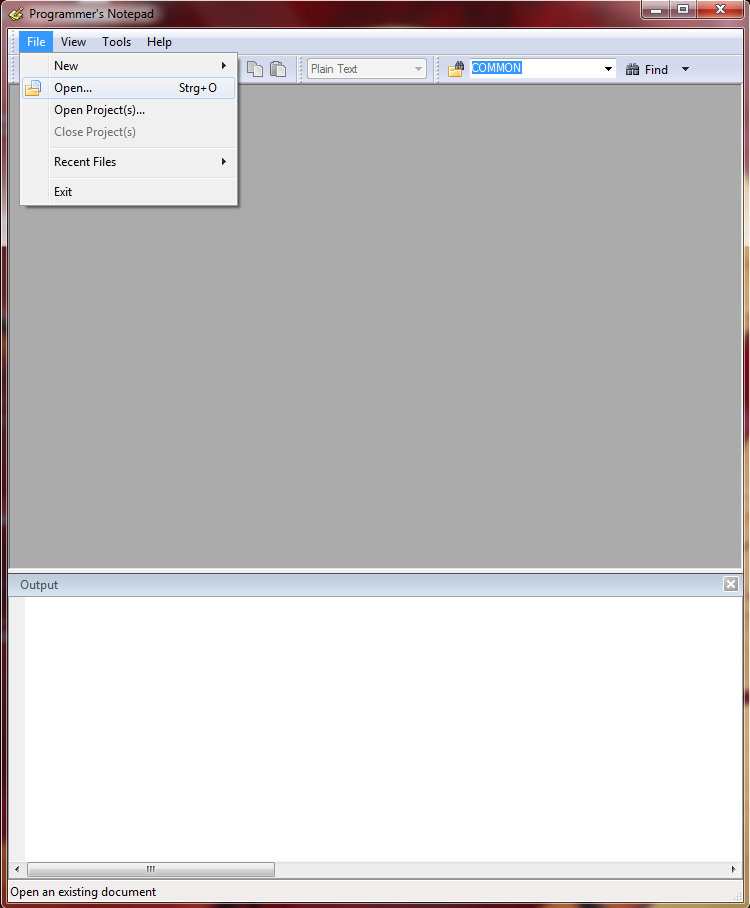
\includegraphics[width=9cm]{../PNG/Notepad_open.png}
    \caption{open Makefile}
  \end{subfigure}
  ~
  \begin{subfigure}[b]{9cm}
    \centering
    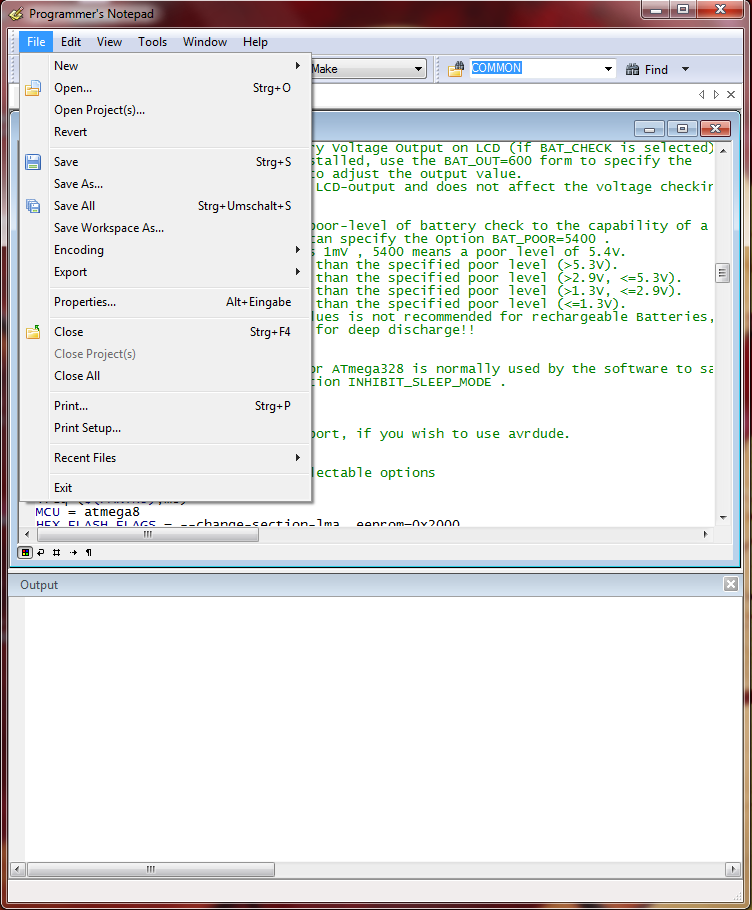
\includegraphics[width=9cm]{../PNG/Notepad_save.png}
    \caption{save Makefile}
  \end{subfigure}
  \caption{Using of the WinAVR user interface Programmer's Notepad}
  \label{fig:WinAVR1}
\end{figure}

The next figures \ref{fig:WinAVR2} show the Tools menu of the Programmer's Notepad
for compiling the program (Make All) and for programming the ATmega (Program) with avrdude.

\begin{figure}[H]
  \begin{subfigure}[b]{9cm}
    \centering
    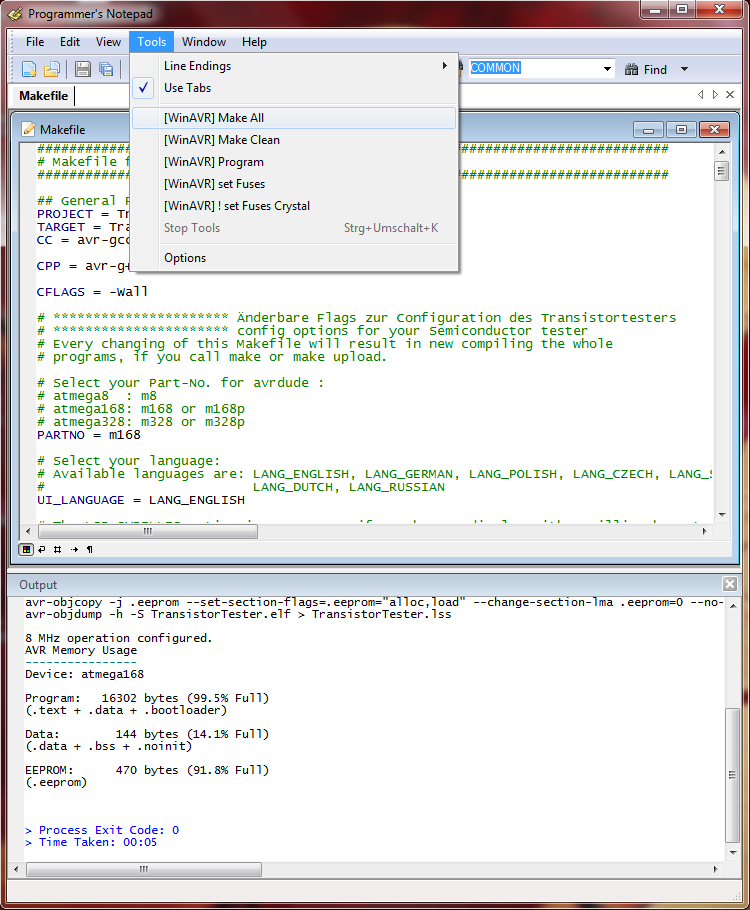
\includegraphics[width=9cm]{../PNG/Notepad_make.png}
    \caption{Build programming data (.hex/.eep)}
  \end{subfigure}
  ~
  \begin{subfigure}[b]{9cm}
    \centering
    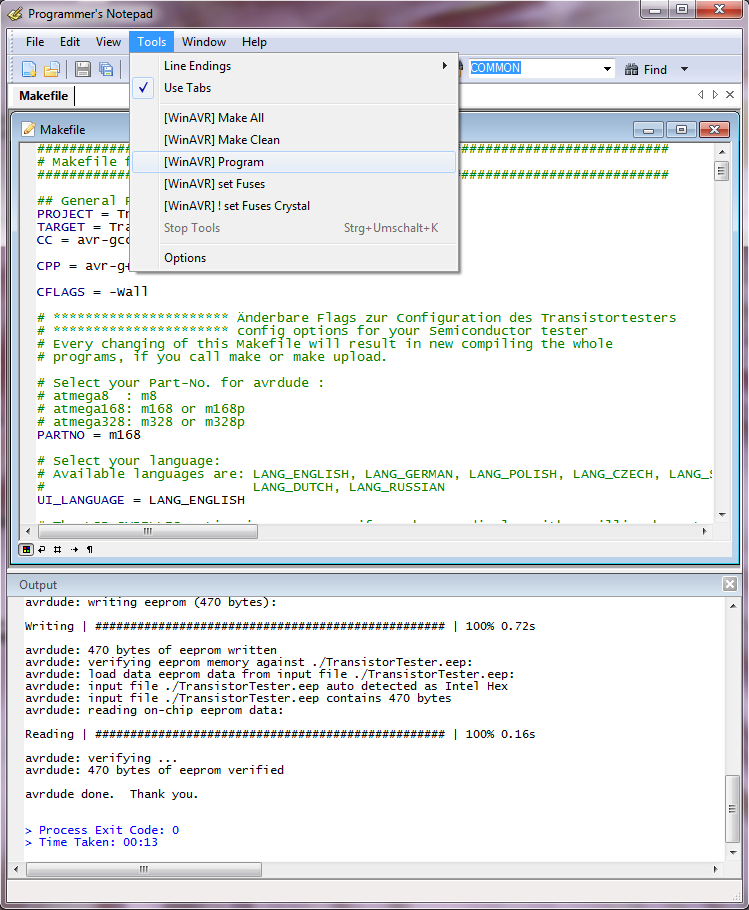
\includegraphics[width=9cm]{../PNG/Notepad_program.png}
    \caption{Programming the ATmega}
  \end{subfigure}
  \caption{Using of the WinAVR user interface Programmer's Notepad}
  \label{fig:WinAVR2}
\end{figure}



\section{Troubleshooting}
In most cases of problems you will miss the text output to the LCD-display.
At first you should check, if the LED was illuminated weak, if you release
the Test button. 
\begin{description}

\item[Power does not switch on.]
If the LED is without light and the VCC power has correct
5V voltage during holding the Test button, the microcontroller does not switch the power
correctly. The microcontroller should hold the power by switching the
PD6 output to 5V, which is usually done as one of the first actions.
If you hold the Test key pressed, the power is switched on anyway.
So you can check the value of VCC power and additionally the voltage value
of the PD6 output, if you hold the key pressed.
If VCC voltage has correct value (5V), but PD6 voltage is
below 4V, your microcontroller does not start the program. In this case
you should check if the microcontroller flash has been loaded with proper data for your
installed type and if ATmega is correctly configured with the fuses.
If your ATmega put the PD6 output to 5V and the power does not stay if you
release the Test key, it is more difficult to find the reason.
First you can shorten the LED and try again. If your Tester now starts,
your LED may be faulty or mounted with wrong polarity. If this is not
the reason, the current amplification factor of your T3 transistor (BC557C)
is insufficient. The current to the base of T3 is lower in the microcontroller
state as in the ``key pressed'' state.

\item[Nothing is readable on the LCD display]
Check the voltage at the contrast pin at the LCD display (pin 3). Adjust to
correct value specified in the data sheet of your display and optimize by viewing.
If you have a high temperature display type, you must provide a negative contrast voltage
for operation. In this case you can use the ICL~7660 device for generating
a negative voltage from positive 5V.

If there is no output readable on the LCD and the background light is on,
you should disconnect the power and check all four data plus the two control signal connections.
If all connection are well, the only reason I see is a uncorrect timing of
control signals. This can be caused by a slower LCD controller than expected by
the software or the ATmega software runs at wrong clock speed. Please check for which
clock speed your programming data was compiled  and if the fuses of the
ATmega are correct set to that speed. You find the clock parameter in the corresponding
Makefile.
If the tester is build without the switch off electronic, you can test with
a LED connected to the test pins, if the program operates normally.
If the LED flickers, the program operates well. The missing text on the
LCD must be caused by wrong connection or timing.


\item[Something but not all is readable on the LCD display]
Check if the .eep data are loaded to the EEprom memory of ATmega.
If all data are loaded correctly, you should check the clock speed of your
programming data (Makefile) and ATmega processor settings (fuses).

\item[Measurement is slow and Capacitors are measured about 8 times too small]
You run software compiled for 8MHz clock at real clock speed of 1MHz.
Please set the fuses of the ATmega correctly.

\item[Measurement has strangely values]
Check if your programmer is still connected to the ISP-plug.
The ISP interface should be disconnected for measuring.
Very often the reason of wrong measurements is the use of software compiled with
the AUTOSCALE\_ADC option and with the option NO\_REF\_CAP, but the capacitor
at the AREF pin has still a value of 100nF.
Wrong assembly of components or remaining soft solder flux can disturb the 
measurements too. Please check with the selftest function of your TransistorTester software
if possible. For the details see Chapter \ref{sec:selftest}.

Otherwise inspect your board visually and check the resistor values
with a ohmmeter. You can use the pins of the ATmega for this check, for example
to check the R1 you can measure between pin 23 and pin 14. Take a look at the
circuit diagram \ref{fig:ttester} for details. There is no need to
remove the microcontroller, only battery or power supply should be removed before.

\item[The Tester switch off the power after 2 seconds display time] 
This condition exists, if the external Pull-Up resistor at the PD7 input
is missing or the key button is keep pressed.
The software switch off the internal Pull-Up resistors to prevent a influence
to the measurement results. Therefore a external Pull-Up resistor (27k) is required.

\item[Der Tester shows only Vext=xx.xV in row 2]
This problem exists, if the Pull-Up resistor at the PD7 input
is missing or the key button is keep pressed.
Additionally the software is configured without the serial output (without option WITH\_UART) and
without the internal Pull-Up resistors (with option PULLUP\_DISABLE).
You should install the Pull-Up resistor at pin PD7.


\end{description}
